% THIS IS AN EXAMPLE DOCUMENT FOR VLDB 2012
% based on ACM SIGPROC-SP.TEX VERSION 2.7
% Modified by  Gerald Weber <gerald@cs.auckland.ac.nz>
% Removed the requirement to include *bbl file in here. (AhmetSacan, Sep2012)
% Fixed the equation on page 3 to prevent line overflow. (AhmetSacan, Sep2012)
 
\documentclass{vldb}
\usepackage{graphicx}
\usepackage{balance}  % for  \balance command ON LAST PAGE  (only there!)
\usepackage{amssymb}
\usepackage{graphicx}
\usepackage{float}
\usepackage{subfigure}
\usepackage{mathtools}
\usepackage{eurosym}

\usepackage{pgfplots}
\usepackage{url}
\usepackage{enumitem}
\usepackage[linesnumbered,ruled]{algorithm2e}
\usepackage[export]{adjustbox}
\usepackage{xspace}
\usepackage{breqn}

%\newcommand{\sgg}{{\sc PolyGuide}}
\newcommand{\sgg}{{\sc GeoPoly}}

% Include information below and uncomment for camera ready
%\vldbTitle{Towards Implicit Feedback Capturing on Spatial Data}
\vldbTitle{Polygon-based Feedback Capturing on Spatial Data}
\vldbAuthors{Behrooz Omidvar-Tehrani, Pl\'acido A. Souza Neto, Tiago Oliveira Lisboa, Francisco B. Silva Junior, Felipe F. Pontes}
\vldbDOI{https://doi.org/TBD}

\begin{document}

% ****************** TITLE ****************************************

%\title{Towards Implicit Feedback Capturing on Spatial Data}
\title{Polygon-based Feedback Capturing on Spatial Data}


% possible, but not really needed or used for PVLDB:
%\subtitle{[Extended Abstract]
%\titlenote{A full version of this paper is available as\textit{Author's Guide to Preparing ACM SIG Proceedings Using \LaTeX$2_\epsilon$\ and BibTeX} at \texttt{www.acm.org/eaddress.htm}}}

% ****************** AUTHORS **************************************

% You need the command \numberofauthors to handle the 'placement
% and alignment' of the authors beneath the title.
%
% For aesthetic reasons, we recommend 'three authors at a time'
% i.e. three 'name/affiliation blocks' be placed beneath the title.
%
% NOTE: You are NOT restricted in how many 'rows' of
% "name/affiliations" may appear. We just ask that you restrict
% the number of 'columns' to three.
%
% Because of the available 'opening page real-estate'
% we ask you to refrain from putting more than six authors
% (two rows with three columns) beneath the article title.
% More than six makes the first-page appear very cluttered indeed.
%
% Use the \alignauthor commands to handle the names
% and affiliations for an 'aesthetic maximum' of six authors.
% Add names, affiliations, addresses for
% the seventh etc. author(s) as the argument for the
% \additionalauthors command.
% These 'additional authors' will be output/set for you
% without further effort on your part as the last section in
% the body of your article BEFORE References or any Appendices.

\numberofauthors{3} %  in this sample file, there are a *total*
% of EIGHT authors. SIX appear on the 'first-page' (for formatting
% reasons) and the remaining two appear in the \additionalauthors section.

\author{
% You can go ahead and credit any number of authors here,
% e.g. one 'row of three' or two rows (consisting of one row of three
% and a second row of one, two or three).
%
% The command \alignauthor (no curly braces needed) should
% precede each author name, affiliation/snail-mail address and
% e-mail address. Additionally, tag each line of
% affiliation/address with \affaddr, and tag the
% e-mail address with \email.
%
% 1st. author
\alignauthor
Behrooz Omidvar-Tehrani\\
       \affaddr{University of Grenoble Alpes (France)}\\
       \email{behrooz.omidvar-tehrani@univ-grenoble-alpes.fr}
% 2nd. author
\alignauthor
Pl\'acido A. Souza Neto\\
       \affaddr{Federal Institute of Rio Grande do Norte (Brazil)}\\
       \email{placido.neto@ifrn.edu.br}
% 3rd. author
\alignauthor
Tiago Oliveira Lisboa\\
       \affaddr{Federal Institute of Rio Grande do Norte (Brazil)}\\
       \email{tiago.oliveira@\\academico.ifrn.edu.br}
\and
% 4th. author
\alignauthor
Francisco B. Silva Junior\\
       \affaddr{Federal Institute of Rio Grande do Norte (Brazil)}\\
       \email{bento.francisco@\\academico.ifrn.edu.br}
% 5th. author
\alignauthor
Felipe F. Pontes\\
       \affaddr{Federal Institute of Rio Grande do Norte (Brazil)}\\
       \email{freire.pontes@\\academico.ifrn.edu.br}
}

\maketitle


\begin{abstract}
Nowadays, spatial data are ubiquitous in various fields of science, such as transportation and social science. Discovering spatial patterns and trends provides improved insights into planning and decision making in various applications such as smart city management. A recent research direction in analyzing spatial data is to provide means for ``exploratory analysis'' of such data where analysts are guided towards interesting options in consecutive analysis iterations. Typically, the guidance component learns analyst's preferences using her explicit feedback, e.g., picking a spatial point or selecting a region of interest. However, it is often the case that analysts forget or don't feel necessary to explicitly express their feedback in what they find interesting. In this paper, we propose \sgg, an approach to capture implicit feedback on spatial data. The approach consists of observing mouse moves (as a means of analyst's interaction) in order to discover interesting spatial regions where the analyst has frequent mouse hovers. For an efficient discovery, we extend ST-DBSCAN and introduce a polygon-based abstraction layer for captured interactions. Using interesting regions, we highlight few points for the analyst to guide her in the analysis process. While we show the process of \sgg\ through a realistic example, we also briefly report on its efficiency and effectiveness.
\end{abstract}

\newpage
\section{Introduction}
Nowadays, there has been a meteoric rise in the generation of spatial datasets in various fields of science, such as transportation, lodging services and social science. As each record in spatial data represents an activity in a precise geographical location, analyzing such data enables discoveries grounded on facts. Analysts are often interested to observe spatial patterns and trends to improve their decision making process. Spatial data analysis has various applications such as smart city management, disaster management and autonomous transport \cite{RoddickEHPS04,Telang:2012}.

\vspace{2pt}
Typically, spatial data analysis begins with an imprecise question in the mind of the analyst, i.e., {\em exploratory analysis}. The analyst requires to go through several trail-and-error iterations to improve her understanding of the spatial data and gain insights. Each iteration involves visualizing a subset of data on geographical maps using an  off-the-shelf product (e.g., Tableau\footnote{\it http://www.tableau.com}, Exhibit\footnote{\it http://www.simile-widgets.org/exhibit/}, Spotfire\footnote{\it http://spotfire.tibco.com}) where the analyst can investigate on different parts of the visualization by zooming in/out and panning on the map. 

\vspace{3pt}
Spatial data are often voluminous. Hence the focus in the literature of spatial data analysis is on ``efficiency'', i.e., enabling fluid means of navigation in spatial data to facilitate the exploratory analysis. The common approach is to design pre-computed indexes which enable efficient retrieval of spatial data (e.g., \cite{lins2013nanocubes}). However, there has been fewer attention to the ``value'' derived from spatial data. Despite the huge progress on the efficiency front, an analyst may easily get lost in the plethora of geographical points due to two following reasons.

\vspace{3pt}
\noindent $\blacksquare$ In an exploratory context, the analyst doesn't know apriori what to investigate next.

\vspace{2pt}
\noindent $\blacksquare$ Moreover, she may easily get distracted and miss interesting points by visual clutter caused by huge point overlaps.

\vspace{3pt}
The main drawback of the traditional analysis model is that the analyst has a {\em passive role} in the process. In other words, the analyst's feedback (i.e., her likes and dislikes) is ignored and only the input query (i.e., her explicit request) is served. In case feedback is incorporated, the process can be more directed towards analyst's interests where her partial needs can be served earlier in the process. In this paper, we advocate for a ``guidance layer'' on top of the raw visualization of spatial data to enable analysts know {\em ``what to see next''}. This guidance should be a function of analyst feedback: the system should recommend options similar to what the analyst has already appreciated. 
% Hence, feedback capturing lies at the core of such guidance system.

\vspace{2pt}
Various approaches in the literature propose methodologies to incorporate analyst's feedback in the exploration process of spatial data. Typically, feedback is considered as a function which is triggered by any analyst's action on the map. The action can be ``selecting a point'', ``moving to a region'', ``asking for more details'', etc. The function then updates a ``profile vector'' which keeps tracks of analyst's interests. The updated content in the profile vector enables the guidance functionality. For instance, if the analyst shows interest in a point which describes a house with balcony, this choice of amenity will reflect her profile to prioritize other houses with balcony in future iterations.

\vspace{2pt}
Feedback is often expressed {\em explicitly}, i.e., the analyst clicks on a point and mentions if she likes or dislikes the point \cite{kamat2014distributed,Omidvar-Tehrani:2015,omidvar2017geoguide}. In \cite{omidvar2017geoguide}, we proposed an interactive approach to exploit such feedback for enabling a more insightful exploration of spatial data. However, there are several cases that the feedback is expressed {\em implicitly}, i.e., the analyst does not explicitly click on a point, but there exists correlations with other signals captured from the analyst which provide hint on her interest. For instance, it is often the case in spatial data analysis that analysts look at some regions of interest but do not provide an explicit feedback. Another example is frequent mouse moves around a region which is a good indicator of the analyst's potential interest in the points in that region. Implicit feedbacks are more challenging to capture and hence less investigated in the literature. The following example describes a use case of implicit feedbacks. This will be our running example which we follow thoughout the paper.

\vspace{2pt}
\noindent {\bf Example.} {\em Ben\'icio is planning to live in Paris for a season. He decides to rent a home-stay from Airbnb website\footnote{\it http://www.airbnb.com}. He likes to discover the city, hence he is open to any type of lodging in any region with an interest to stay in the center of Paris. The website returns 1500 different locations. As he has no other preferences, an exhaustive investigation needs scanning each location independently which is nearly infeasible. While he is scanning few first options, he shows interest in the region of Trocadero (where the Eiffel tower is located in) but he forgets or doesn't feel necessary to click a point there. An ideal system should capture this implicit feedback in order to short-list a small subset of locations that Ben\'icio should consider as high priority}.

\vspace{2pt}
The above example shows in practice that implicit feedback capturing is crucial in the context of spatial data analysis. While text-boxes, combo-boxes and other input elements are available in analyzing other types of data, the only interaction means between the analyst and a spatial data analysis system is a geographical map spanned on the whole screen. In this context, a point can be easily remained out of sight and missed.

\vspace{2pt}
In this paper, we present an approach called {\sc GeoPoly} whose aim is to capture and analyze implicit feedback of analysts in spatial data analysis. Without loss of generality, we focus on ``mouse moves'' as the implicit feedback received from the analyst. Mouse moves are the most common way that analysts interact with geographical maps~\cite{Chen:2001}. It is shown in \cite{Arapakis:2014} that mouse gestures have a strong correlation with ``user engagement''. Intuitively, a point gets a higher weight in the analyst's profile if the mouse cursor moves around it frequently.  However, our approach can be easily extended to other types of inputs such gaze tracking, leap motions, etc.

% \cite{Robertson2007}  affirms that temporal change in spatial patterns are increasingly common in geographical analysis. This work explore an approach to the spatialtemporal analysis of polygons that are spatially distinct and experience discrete changes though time. It presents challenges considering changes of regions (polygons) during the time. Works like \cite{Ester:1996} and  \cite{Birant:2007} present solutions for clustering spatialtemporal data. These solutions are relevant to define regions by each cluster that contains important informations for the user. 

% \vspace{3pt}
% Discovering patterns and provide tendencies in spatial data applications may improve insights for planning and decision making for smart city solutions. Many systems and datasets consider space information.  In this way, find spatial preferences can offer interactive and guidance solutions.  For example,  when users look for a house or hotel to spend a season, they consider one or more regions of their preference. These regions are intrinsic to each user, or user group. However, when navigating the application, the user also considers regions that seem interesting, for different reasons, such as the priority of some tourist spot, restaurants, clubs, security, etc. Thus, capturing region preferences over time can help to guide the user to find better places.
 
% \vspace{3pt}
% Given a dataset of spatial points and from the mouse tracking movements by the user, our approach generates a set of highlighted regions based on its preferences. Each region is related with a subset of highlighted points which are illustrated using visual variables such as size and color intensity. The regions are also highlighted.

\vspace{2pt}
The outline of the paper is the following. Section \ref{sec:datamodel} describes our data model. In Section \ref{sec:problem}, we formally define our problem. Then in Section \ref{sec:algo}, we present our solution and its algorithmic details. Section  \ref{sec:exp} reports our experiments on the framework. We review the related work in Section \ref{sec:rel}. Last, we conclude in Section \ref{sec:conc}.
\section{Data Model}\label{sec:data-model}
% prune this
A wide range of spatiotemporal data is present in a vast variety of datasets such as aviation, ground transportation (bike, taxi, renting- car, bus), urban data, geo-tagged social networks, crimes, events, etc. Intuitively, the common point between all those dataset is having {\em location} and {\em time} attributes. Based on this particularity, we propose a generic data model to capture all diverse aspects of such data.

We consider a spatiotemporal database ${\cal D}$ consisting $\langle {\cal P}, {\cal A} \rangle$ where ${\cal P}$ is the set of
geographical points and ${\cal A}$ is the set of point attributes. For each $p \in {\cal P}$, we consider a tuple $<id, lat, lon, alt, t>$ where $id$ is the point identifier, $lat$, $lon$ and $alt$ denote $p$'s geographical coordinates (latitude, longitude and altitude respectively), and $t$ is the timestamp.

The set ${\cal A}_p$ contains attribute-values for $p$ over the schema of ${\cal A}$. For instance, on a bike-sharing dataset, ${\cal A}_p = \langle $ {\tt female}, {\tt young}, {\tt subscribed} $\rangle$ on the schema ${\cal A} = \langle$ {\tt gender}, {\tt age-category}, {\tt subscription} $\rangle$ denotes that $p$ is associated to a young female cyclist who is subscribed in the bike-sharing system. The set ${\cal A}$ is domain-dependent and defines the semantics of a spatiotemporal dataset. For instance, in case of a taxi dataset, ${\cal A} = \langle$ {\tt dropoff\_time}, {\tt price}, {\tt tip} $\rangle$, where for an aviation dataset, ${\cal A} = \langle$ {\tt aircraft\_type}, {\tt departure\_airport}, {\tt arrival\_airport} $\rangle$.

% prune this
Some spatiotemporal datasets contain point-sets as entities, such as {\em trajectories} in transportation datasets and {\em regions} in urban or agriculture dataset. Although our generic data model only captures the finest granular concept (i.e., point), we define ${\cal S}$ containing point-sets. Each point-set $s \in {\cal S}$ is indeed a set of points where $s \subseteq {\cal P}$. For instance, in a taxi dataset, $s = [ p_1, p_2 \dots p_n ]$ shows a ride consisting $n$ points departing at $p_1$ and arriving at $p_n$.
\section{Problem Statement}
\label{sec:pb}
% In an exploratory analysis context, the analyst does not necessarily know what to ask. She may have also a few knowledge about the spatiotemporal data and its attributes. Hence she usually needs to take iterative analysis steps to observe different aspects of data and ultimately land on a subset of interest. However, it is often cumbersome to choose what to analyze next. Because this choice is subjective and infeasible to capture with an unsupervised method.

In this paper, we address the problem of {\em generic guidance} in spatiotemporal data: ``what is the process of guiding analysts in iterative analysis steps on any spatiotemporal dataset?'' In other words, we are interested in an approach which highlights a set of $k$ points that the analyst should consider in the next analysis iteration. This should not be a heuristic-based data-dependent highlighting, but a generic approach which is applied on any spatiotemporal dataset. We describe the desiderata of generic guidance approach as follows.

\vspace{5pt}
\noindent {\bf D1. Genericness.} The guidance component should be agnostic (making no assumption) about the dataset type, attributes and distribution.

\vspace{5pt}
\noindent {\bf D2. Limited Options.} The set of $k$ highlighted points should not be very large because too many options distract the analyst. % \cite{miller1956human}.

\vspace{5pt}
\noindent {\bf D3. Relevance.} The fundamental difference between highlighting and $k$-NN spatial queries \cite{aly2015spatial} is that, in the former, the focus is on $k$ points which have similar characteristics to $p$, hence relevant.
% In other words, we are interested in points which are {\em relevant} to a given point of interest.
For instance, consider a taxi ride in New York for a young male customer for an itinerary of 10 kilometers and \$3 tip. In contrary to thousands of kilometers of geographical distance, the ride is very similar to another one in San Fransisco for a middle-age male customer for an itinerary of 8 kilometers and \$2.5 tip.
% Relevance is a pairwise metric which is associated to point characteristics.
Given two points $p$ and $p'$, we define {\em relevance} as follows.

% \begin{definition}[Relevance]
% Given two points $p$ and $p'$ and their attribute values ${\cal A}_{p}$ and ${\cal A}_{p'}$, the relevance between $p$ and $p'$ is a value between $0$ and $1$ denoted as $\mathit{relevance}(p,p') = \mathit{average}_{a \in {\cal A}_{p} \cup {\cal A}_{p'}}(\mathit{sim({\cal A}_{p}, {\cal A}_{p'}, a)})$.
% \label{def:rel}
% \end{definition}

\begin{dmath}
\label{eq:rel}
\mathit{relevance}(p,p') = \mathit{average}_{a \in {\cal A}_{p} \cup {\cal A}_{p'}}(\mathit{sim(p, p', a)})
\end{dmath}

The similarity function $\mathit{sim}()$ can be any function such as Jaccard and Cosine. Each attribute can have its own similarity function (as string and integer attributes are compared differently.) Then $\mathit{sim}()$ works as an overriding-function which provides encapsulated similarity computations for any type of attribute.

\vspace{5pt}
\noindent {\bf D4. Diversity.} A guidance approach should also consider coverage of all points: $k$ highlighted points should represent distinct regions so that the analyst can observe different aspects of data and decide for the next analysis iteration. Hence, $k$ points should be diverse.
% Diversity is a set-based metric and is associated to geographical distance. We define this metric as follows.
Given a set of points $s = \{ p_1, p_2 \dots \}$, we define {\em diversity} as follows.

\begin{dmath}
\label{eq:divs}
\mathit{diversity}(s) = \mathit{average}_{\{p, p'\} \subseteq s | p \neq p' } \mathit{distance}(p,p')
\end{dmath} 

The function $\mathit{distance}(p,p')$ operates on geographical coordinates of $p$ and $p'$ and can be considered as any distance function of Chebyshev distance family such as Eucledian. However, as distance computations are done in {\em spherical space} using latitude, longitude and altitude, it is au-naturel to employ Harvestine distance shown in Equation \ref{eq:harvestine}.

\begin{dmath}
\label{eq:harvestine}
distance(p,p') = [ acos(cos(p_{lat}) . cos(p'_{lat}) . cos(p_{lng}) . cos(p'_{lng})\\ + cos(p_{lat}) . sin(p'_{lat}). cos(p_{lng}) . sin(p'_{lng}) + sin(p_{lat}) . sin(p'_{lat})) ] \times earth\_radius
\end{dmath}

\noindent {\bf D5. Interactivity.} The exploratory nature of the analysis requires the guidance component to be involved in an interactive process. Hence the analyst can investigate and refine different aspects of spatiotemporal data in iterative steps. For being interactive, the guidance component should be efficient so that the train of thought of analyst would not be broken during the analysis process.

\vspace{5pt}
Following aforementioned desiderata, we forumlate highlighting as an optimization-based problem where we optimize diversity and respect a bound on relevance.

\begin{problem}[\pb]
\label{pb:geoh}
Given an input point $p$ and a threshold $\sigma$, the problem is to return $k$-relevant points to $p$ denoted $S_p$ where $|S_p| = k$ and $\forall p' \in S_p, \mathit{relevance}(p,p') \geq \sigma$ and $\mathit{diversity}(S_p)$ is maximized.
\end{problem}

Problem \ref{pb:geoh} is hard due to the huge space of spatiotemporal data: for any given point $p$, an exhaustive search over all other points is necessary to find $k$ points with maximal relevance. Moreover, the problem expresses interest in obtaining high quality points in two dimensions at the same time (relevance and diversity) which makes the problem more challenging.

% behrooz: talk about quality earlier
\newpage
\section{GeoPoly Framework}
\label{sec:algo}
{\sc GeoPoly} is an approach which exploits analyst's implicit feedback (i.e., mouse moves) to highlight few interesting points as future analysis directions. Algorithm \ref{algo:main} summarizes the principled steps of our approach.

\begin{algorithm}[t]
\DontPrintSemicolon
\KwIn{Current time $t_c$, mouse move points $\mathcal{M}$}
\KwOut{Highlights $\mathcal{P}_k$}
$\mathcal{S} \gets \mathit{find\_interesting\_dense\_regions}(t_c,\mathcal{M})$\label{ln:dense}\;
$\mathcal{P}_s \gets \mathit{match\_points}(\mathcal{S}, \mathcal{P})$\label{ln:match}\;
$F \gets \mathit{update\_feedback\_vector}(F, \mathcal{P}_s)$\label{ln:update}\;
$\mathcal{P}_k \gets \mathit{get\_highlights}(\mathcal{P}, F)$\label{ln:highlight}\;
\Return{$\mathcal{P}_k$}\; 
\caption{{\sc GeoPoly} Algorithm}
\label{algo:main}
\end{algorithm}

\vspace{2pt}
The algorithm begins by mining the set of mouse move points $\mathcal{M}$ in the interaction layer to discover one or several Interesting Dense Regions, abbr., IDRs, in which most analyst's interactions occur (line \ref{ln:dense}). Then it matches the spatial points $\mathcal{P}$ with IDRs using Equation \ref{eq:reverse} in order to find points inside each ragion (line \ref{ln:match}). The attributes of resulting points will be exploited to update the analyst's feedback vector~$F$~(line \ref{ln:update}). The updated vector $F$ will then be used to find $k$ highlights (line \ref{ln:highlight}). These steps ensure that the final highlights reflect analyst's implicit interests. We detail each step as follows.

\subsection{Interesting Dense Regions}
The objective of this step is to obtain one or several regions in which the analyst has expressed her implicit feedback. There are two observations for such regions.

\vspace{2pt}
\noindent $\blacksquare$ {\bf Observation 1.} We believe that a region appeals more interesting to the analyst if it is denser, i.e., the analyst moves her mouse in that region several times.

\vspace{2pt}
\noindent $\blacksquare$ {\bf Observation 2.} It is possible that the analyst moves her mouse everywhere in the map. This should not signify that everywhere in the map has the same significance.

\vspace{2pt}
Following our observations, we propose Algorithm \ref{algo:dense} for mining IDRs. We add points to $\mathcal{M}$ only every $200ms$ to prevent adding redundant points.  Following Observation 1 and in order to mine the recurring behavior of the analyst, the algorithm begins by partitioning the set $\mathcal{M}$ into $g$ fixed-length consecutive segments $\mathcal{M}_0$ to $\mathcal{M}_g$. The first segment starts at time zero (where the system started), and the last segment ends at $t_c$, i.e., the current time. Following Observation 2, we then find dense clusters in each segment of $\mathcal{M}$ using a variant of DB-SCAN~\cite{Ester:1996} approach. Finally, we return intersections among those clusters as IDRs.

\vspace{2pt}
For clustering points in each time segment (i.e., line \ref{ln:mine} of Algorithm~\ref{algo:dense}), we use ST-DBSCAN~\cite{Birant:2007}, a space-aware variant of DB-SCAN for clustering points based on density. For each subset of mouse move points $\mathcal{M}_i$, $i \in [0,g]$, ST-DBSCAN begins with a random point $m_0 \in \mathcal{M}_i$ and collects all density-reachable points from $m_0$ using a distance metric. As mouse move points are the 2-dimensional pixel space (i.e., the display), we choose euclidean distance as the distance metric. If $m_0$ turns out to be a core object, a cluster will be generated. Otherwise, if $m_0$ is a border object, no point is density-reachable from $m_0$ and the algorithm picks another random point in $\mathcal{M}_i$. The process is repeated until all of the points have been processed.

\vspace{2pt}
Once clusters are obtained for all subsets of $\mathcal{M}$, we find their intersections to locate recurring regions (line \ref{ln:poly}). To obtain intersections, we need to clearly define the spatial boundaries of each cluster. Hence for each cluster, we discover its corresponding polygon that covers the points inside. For this aim, we employ Quickhull algorithm, a quicksort-style method which computes the convex hull for a given set of points in a 2D plane~\cite{Barber:1996}.
% We analysed other different approaches~\cite{Bevis1989,DUCKHAM2008,FADILI2004,ARAMPATZIS2006,Galton2006} to generate regions from clustered points, however we decided to use the Quickhull  algorithm~\cite{Barber:1996}, that presented more appropriated to our proposed solution.

\begin{figure*}[t]
\centering
   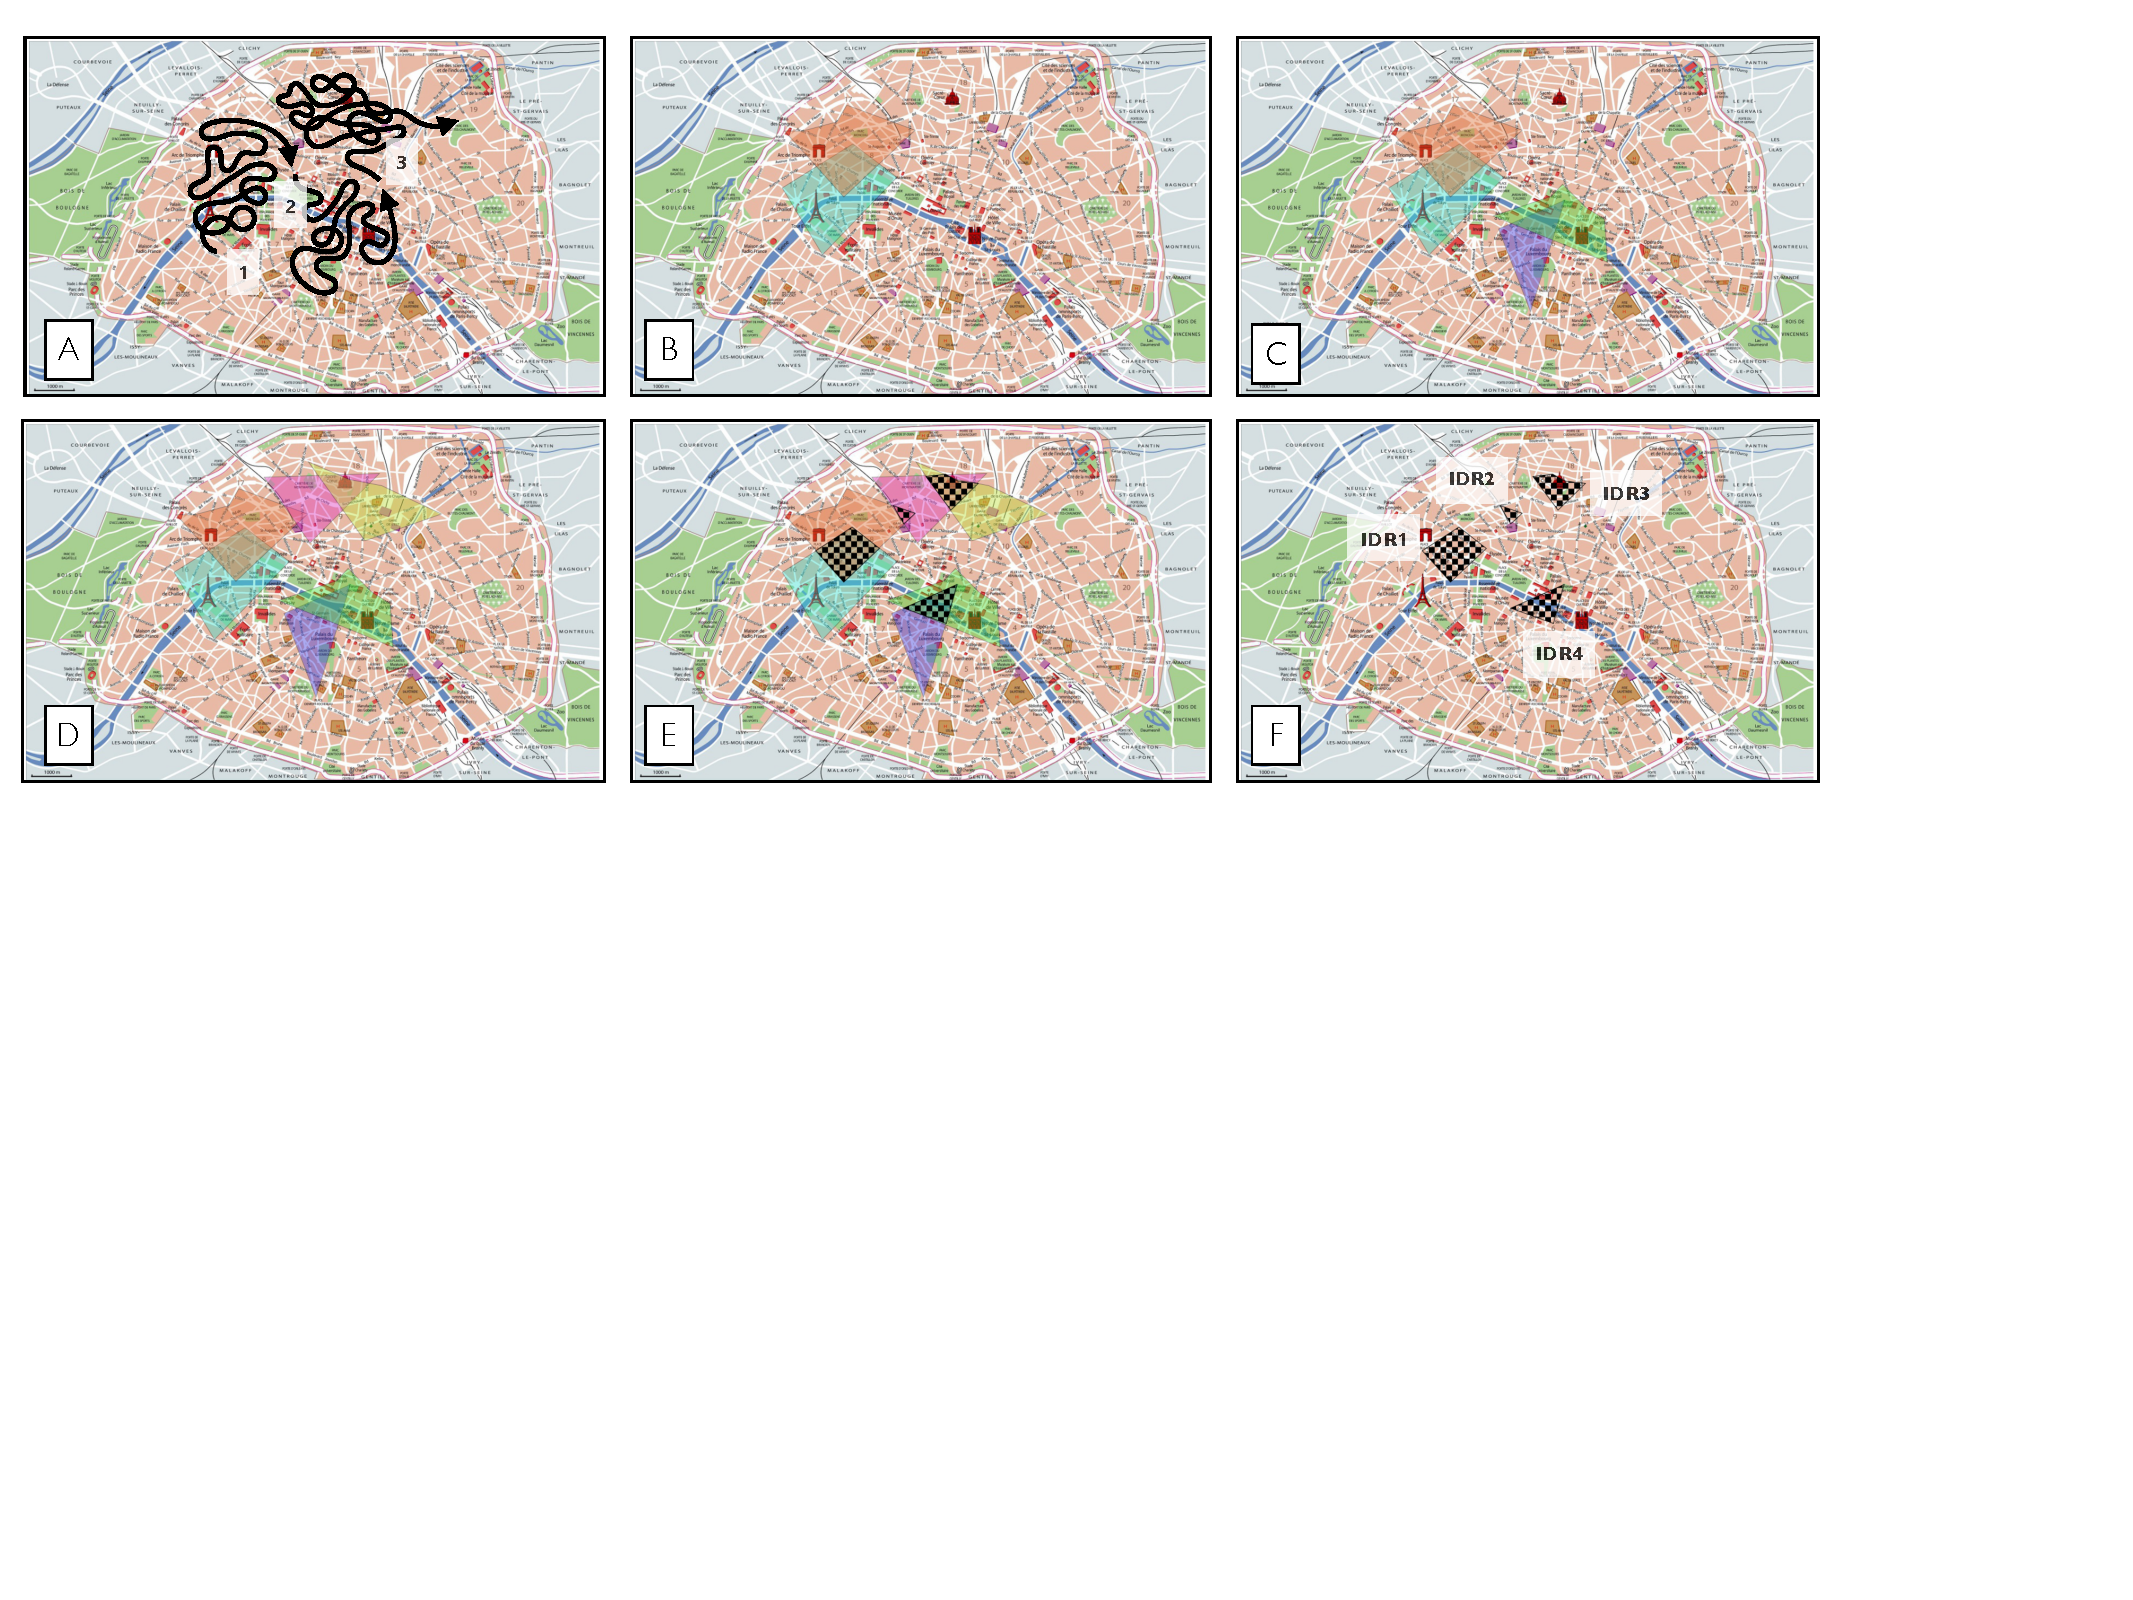
\includegraphics[width=\textwidth]{imgs/regions}
  \caption{The process of finding IDRs on Airbnb dataset.}
  \label{fig:regions}
\end{figure*}

\begin{algorithm}[t]
\DontPrintSemicolon
\KwIn{Current time $t_c$, mouse move points $\mathcal{M}$}
\KwOut{IDRs $\mathcal{S}$}
$\mathcal{S} \gets \emptyset$\;
$g \gets ${\em number of time segments}\;
\For{$i \in [0,g]$}
{
       $\mathcal{M}_i \gets \{m = \langle x,y,t \rangle | (\frac{t_c}{g} \times i) \leq t \leq (\frac{t_c}{g} \times (i+1))\}$\;
       $\mathcal{C}_i \gets \mathit{mine\_clusters}(\mathcal{M}_i)$\label{ln:mine}\;
       $\mathcal{O}_i \gets \mathit{find\_ploygons}(\mathcal{C}_i)$\label{ln:poly}\;
}
\lFor{$\mathcal{O}_i, \mathcal{O}_j$ where $i,j \in [0,g]$ and $i \neq j$}
{
       $\mathcal{S}.\mathit{append}(\mathit{intersect}(\mathcal{O}_i, \mathcal{O}_j))$
}
\Return{$\mathcal{S}$}\; 
\caption{Find Interesting Dense Regions (IDRs)}
\label{algo:dense}
\end{algorithm}

\begin{figure}[t]
\centering
   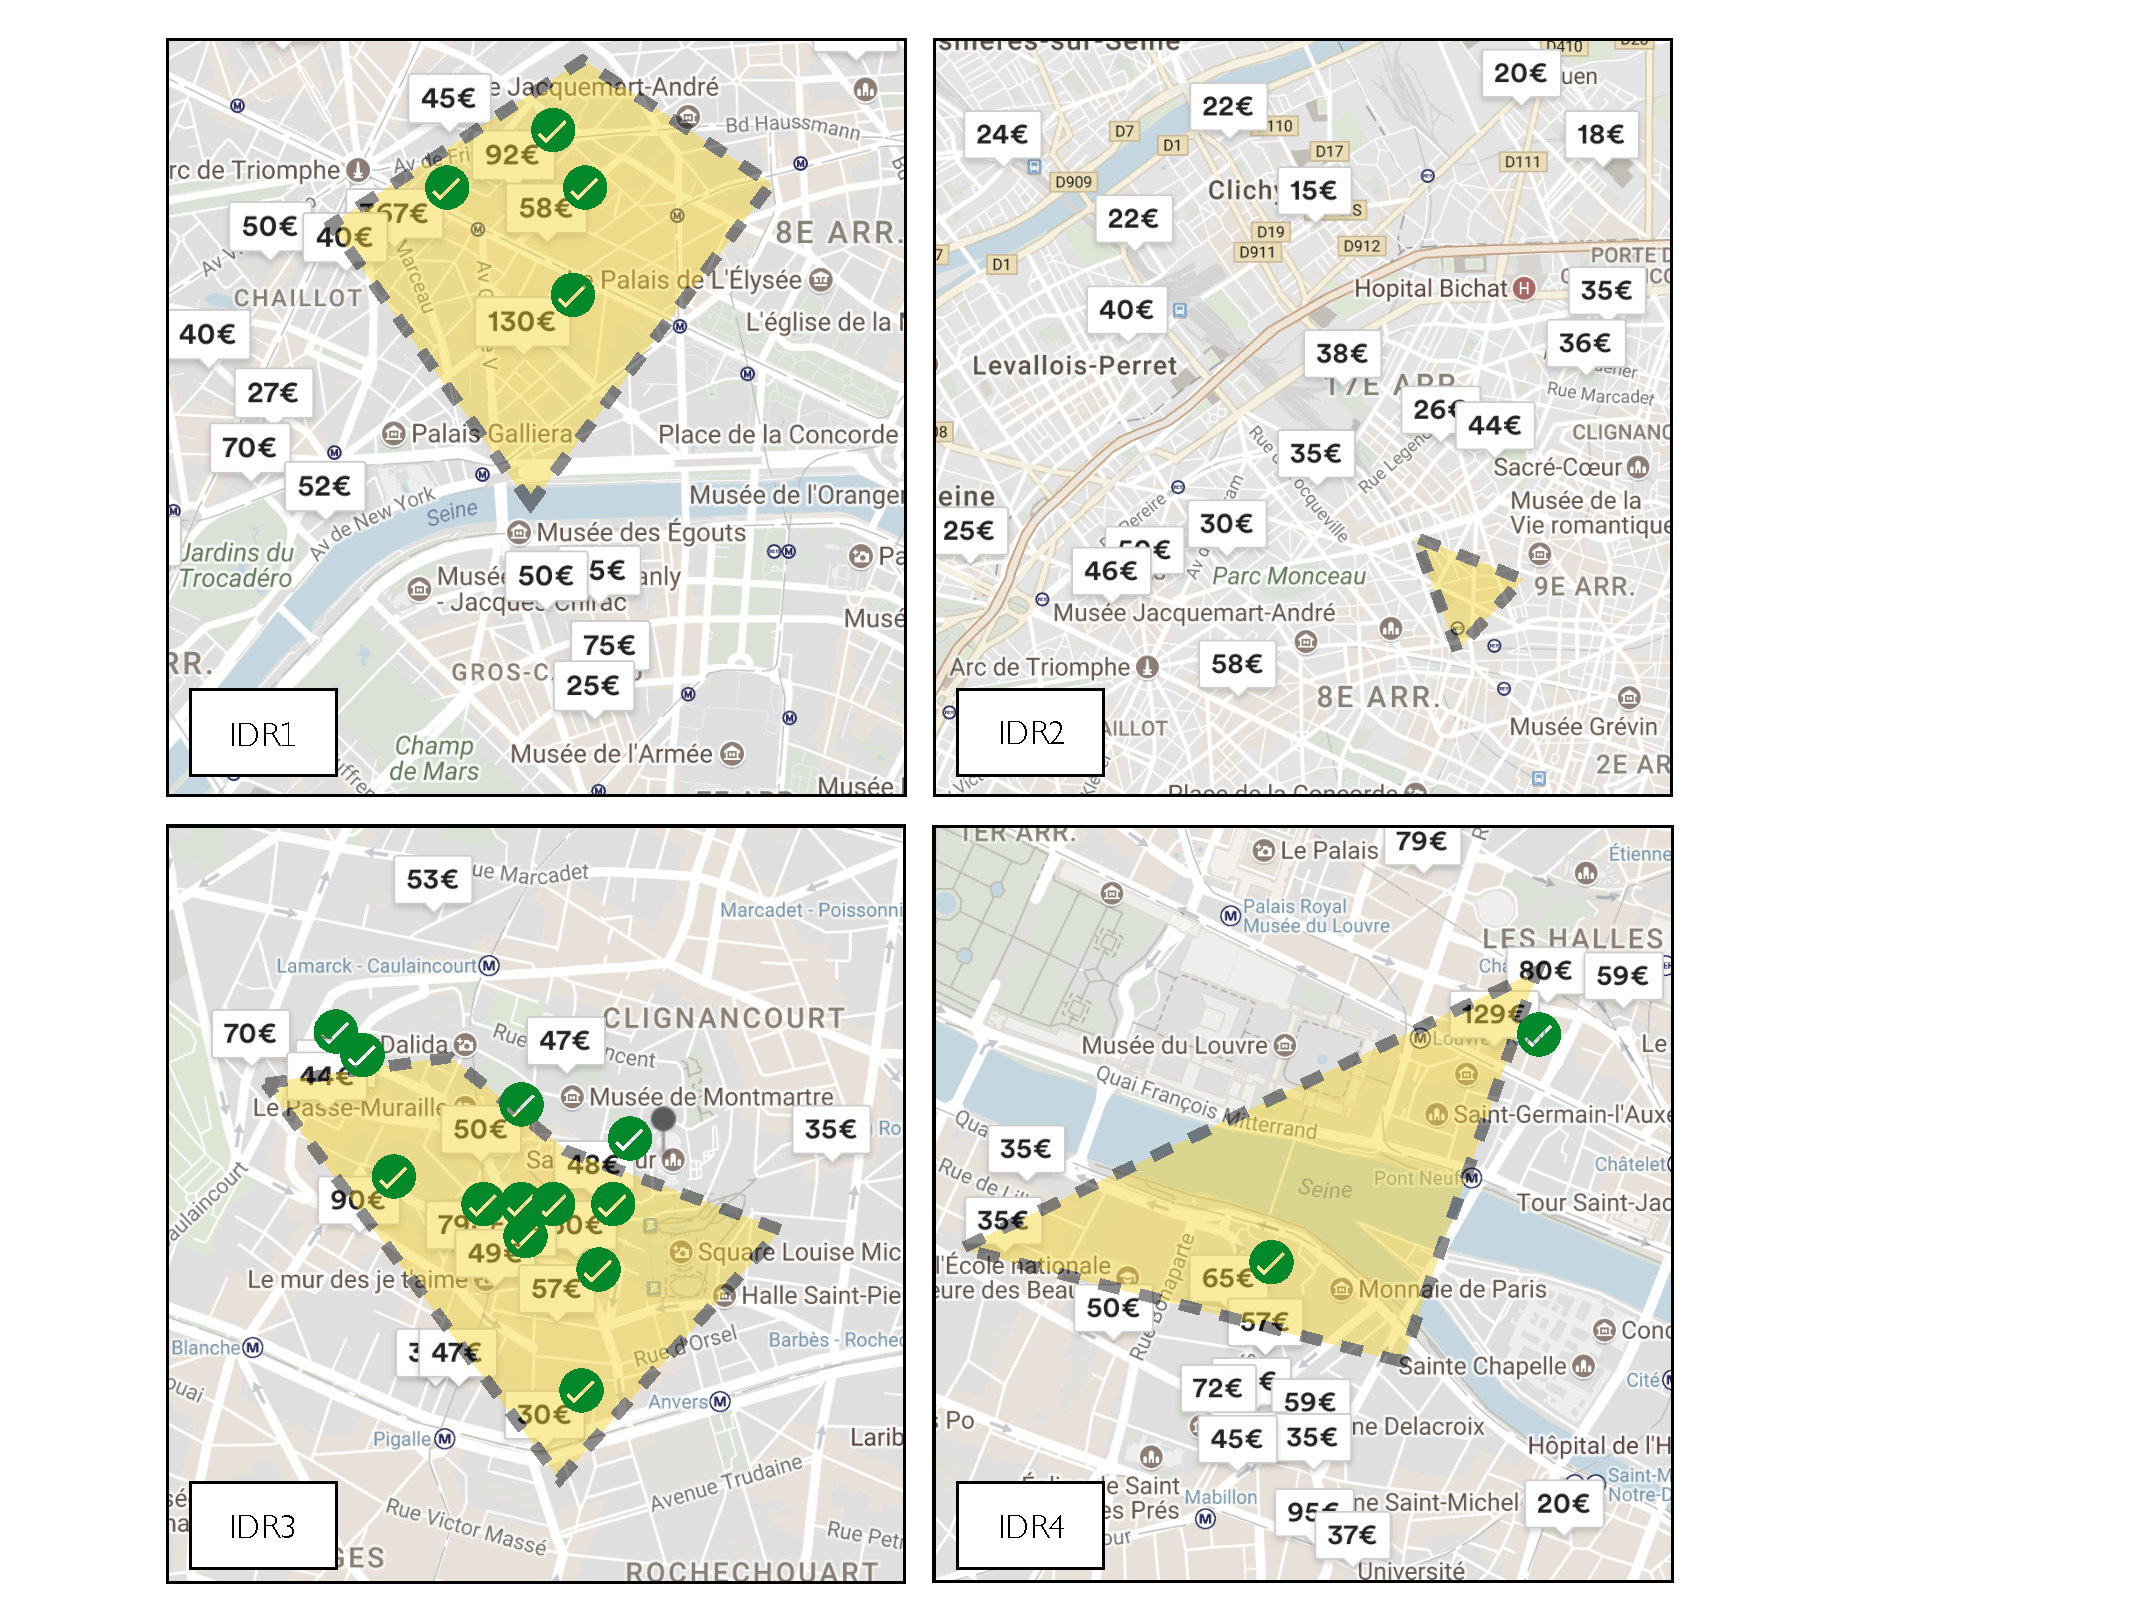
\includegraphics[width=\columnwidth]{imgs/match}
  \caption{Matching points for IDR1 to IDR4.}
  \label{fig:match}
\end{figure}

\vspace{2pt}
We describe the process of finding IDRs in an example. Figure \ref{fig:regions} shows the steps that Ben\'icio follows in our running example to explore home-stays in Paris. Figure \ref{fig:regions}.A shows mouse movements of Ben\'icio in different time stages. In this example, we consider $g = 3$ and capture Ben\'icio's feedback in three different time segments (progressing from Figures \ref{fig:regions}.B to \ref{fig:regions}.D). It shows that Ben\'icio started his search around Eiffel Tower and Arc de Triomphe (Figure \ref{fig:regions}.B) and gradually showed interest in south (Figure \ref{fig:regions}.C) and north (Figure \ref{fig:regions}.D) as well. All intersections between those clusters are discovered (hatching regions in Figure \ref{fig:regions}.E) which will constitute the set of IDRs (Figure \ref{fig:regions}.F), i.e., IDR1 to IDR4.

\subsection{Matching Points}
Being a function of mouse move points, IDRs are discovered in the interaction layer. We then need to find out which points in $\mathcal{P}$ fall into IDRs, hence forming the subset $\mathcal{P}_s$. We employ Equation \ref{eq:reverse} to transform those points from the spatial layer to the interaction layer. Then a simple ``spatial containment'' function can verify which points fit into the IDRs. Given a point $p$ and an IDR $r$, a function $\mathit{contains}(p,r)$ returns ``true'' if $p$ is inside $r$, otherwise ``false''. In our case, we simply use the implementation of $\mathit{ST\_Within}(p,r)$ module in PostGIS\footnote{\it https://postgis.net/docs/manual-dev/ST\_Within.html}, i.e., our underlying spatial DBMS which hosts the data.

\vspace{2pt}
In the vanilla version of our spatial containment function, all points should be checked against all IDRs. Obviously, this depletes the execution time. To prevent the exhaustive scan, we employ Quadtrees in a two-step approach.

\vspace{4pt}
\noindent $\blacksquare$ In an offline process, we build a Quadtree index for all points in $\mathcal{P}$. We record the membership relations of points and cells in the index.

\vspace{2pt}
\noindent $\blacksquare$ When IDRs are discovered, we record which cells in the Quadtree index intersect with IDRs. As we often end up with few IDRs, the intersection verification performs fast. Then for matching points, we only check a subset which is inside the cells associated to IDRs and ignore the points outside. This leads to a drastic pruning of points in $\mathcal{P}$.

\vspace{4pt}
We follow our running example and illustrate the matching process in Figure \ref{fig:match}. In the Airbnb dataset, points are home-stays which are shown with their nightly price on the map. We observe that there exist many matching points with IDR3 and absolutely no matching point for IDR2. For IDR4, although there exist many home-stays below the region, we never check their containment, as they belong to a Quadtree cell which doesn't intersect with the IDR. 

\subsection{Updating Analyst Feedback Vector}
The set of matching points $\mathcal{P}_s$ (line \ref{ln:match} of Algorithm \ref{algo:main}) depicts the implicit preference of the analyst. We keep track of this preference in a feedback vector $F$. The vector is initialized by zero, i.e., the analyst has no preference at the beginning. We update $F$ using the attributes of the points in $\mathcal{P}_s$.

\vspace{2pt}
We consider an {\em increment value} $\delta$ to update $F$. If $p \in \mathcal{P}_s$ gets $v_1$ for attribute $a_1$, we augment the value in the $F$'s cell of $\langle a_1, v_1 \rangle$ by $\delta$. Note that we only consider incremental feedback, i.e., we never decrease a value in $F$.

\vspace{2pt}
We explain the process of updating the feedback vector using a toy example. Given the four matched points in IDR1 (Figure \ref{fig:match}) with prices 130\euro, 58\euro, 92\euro\ and 67\euro, we want to update the vector $F$ given those points. Few attributes of these points are mentioned in Table \ref{tbl:attribs}. In practice, there are often more than 50 attributes for points. The cells of $F$ is illustrated in the first column of Table \ref{tbl:feedback}. As three points get the value ``1'' for the attribute ``\#Beds'', then the value in cell $\langle$\#Beds,1$\rangle$ is augmented three times by $\delta$. The same process is repeated for all attribute-values of points in $\mathcal{P}_s$. Note that all cells of $F$ are not necessarily touched in the feedback update process. For instance, in the above example, 5 cells out of 12 remain unchanged.

\vspace{2pt}
By specifying an increment value, we can materialize the updates and normalize the vector using a Softmax function. We always normalize $F$ in a way that all cell values sum up to $1.0$. Given $\delta = 1.0$, the normalized values of the $F$ vector is illustrated in the third column of Table \ref{tbl:feedback}. Higher values of $\delta$ increase the influence of feedbacks.

\vspace{2pt}
The normalized content of the vector $F$ captures the implicit preferences of the analyst. For instance, the content of $F$ after applying points in IDR1 shows that the analyst has a high interest in having a balcony in her home-stay, as her score for the cell $\langle$Balcony,Yes$\rangle$ is 0.25, i.e., the highest among other cells. This reflects the reality as all points in IDR1 has balcony. Note that although we only consider positive feedback, the Softmax function lowers the values of untouched cells once other cells get rewarded.

\vspace{2pt}
An important consideration in interpreting the vector $F$ is that the value ``0'' does not mean the lowest preference, but {\em irrelevance}. For instance, consider the cell $\langle$Rating,2$\rangle$ in Table \ref{tbl:feedback}. The value ``0'' for this cell shows that the analyst has never expressed her implicit feedback on this facet. It is possible that in future iterations, the analyst shows interest in a 2-star home-stay (potentially thanks to its price), hence this cell gets a value greater than zero. However, cells with lower preferences are identifiable with non-zero values tending to zero. For instance, the value 0.06 for the cell $\langle$Rating,4$\rangle$ shows a lower preference towards 4-star home-stays comparing to the ones with 5 stars, as only one point in $\mathcal{P}_s$ is rated 4 in IDR1.

\begin{table}[t]
\centering
\caption{Attributes of points in IDR1.}
\label{tbl:attribs}
\begin{tabular}{|c|c|c|c|c|c|}
\hline
\textbf{ID} & \textbf{Price} & \textbf{\#Beds} & \textbf{Balcony} & \textbf{Air-cond.} & \textbf{Rating} \\ \hline
1                     & 130\euro           & 1               & Yes           & Yes                & 5/5             \\ \hline
2                     & 58\euro            & 1               & Yes           & No                 & 5/5             \\ \hline
3                     & 92\euro            & 2               & Yes           & No                 & 5/5             \\ \hline
4                     & 67\euro            & 1               & Yes           & No                 & 4/5             \\ \hline
\end{tabular}
\end{table}

\begin{table}[t]
\centering
\caption{Updating Analyst Feedback Vector}
\label{tbl:feedback}
\begin{tabular}{|c|c|c|}
\hline
\textbf{Attribute-value}               & \textbf{Applying IDR 1} & \textbf{Normalized} \\ \hline
$\langle$\#Beds,1$\rangle$                   & $+3\delta$                       & 0.19                 \\ \hline
$\langle$\#Beds,2$\rangle$                 & $+\delta$                       & 0.06                 \\ \hline
$\langle$\#Beds,+2$\rangle$                  & {\em (no update)}                       & 0.00                    \\ \hline
$\langle$Balcony,Yes$\rangle$                   & $+4\delta$                      & {\bf 0.25}                 \\ \hline
$\langle$Balcony,No$\rangle$                    & {\em (no update)}                        & 0.00                    \\ \hline
$\langle$Air-cond.,Yes$\rangle$               & $+\delta$                       & 0.06                 \\ \hline
$\langle$Air-cond.,No$\rangle$                & $+3\delta$                       & 0.19                 \\ \hline
$\langle$Rating,1$\rangle$                    & {\em (no update)}                       & 0.00                    \\ \hline
$\langle$Rating,2$\rangle$                     & {\em (no update)}                        & 0.00                    \\ \hline
$\langle$Rating,3$\rangle$                    & {\em (no update)}                        & 0.00                   \\ \hline
$\langle$Rating,4$\rangle$                   & $+\delta$                       & {\bf 0.06}                 \\ \hline
$\langle$Rating,5$\rangle$                     & $+3\delta$                      & 0.19                 \\ \hline
\end{tabular}
\end{table}

\subsection{Generating Highlights}
The ultimate goal of \sgg\ is to highlight $k$ points to guide analysts in analyzing their spatial data. The updated feedback vector $F$ is the input to the highlighting phase. We assume that points in IDRs are already investigated by the analyst. Hence our search space for highlighting is $\mathcal{P} - \mathcal{P}_s$.

\vspace{2pt}
We seek two properties in $k$ highlights, i.e., {\em similarity} and {\em diversity}. First, highlights should be in the same direction of the analyst's implicit feedback, hence similar to the vector~$F$. The similarity between a point $p \in \mathcal{P}$ and the vector~$F$ is defined as follows.

\begin{equation}
       \label{eq:rel}
       \mathit{similarity}(p,F) = \mathit{avg}_{a \in \mathcal{A}}(\mathit{sim(p, F, a)})
\end{equation}

The $\mathit{sim}()$ function can be any function such as Jaccard and Cosine. Each attribute can have its own similarity function (as string and integer attributes are compared differently.) Then $\mathit{sim}()$ works as an overriding-function which provides encapsulated similarity computations for any type of attribute.

\vspace{2pt}
Second, highlighted points should also represent distinct directions so that the analyst can observe different aspects of data and decide based on the big picture. Given a set of points $\mathcal{P}_k = \{ p_1, p_2 \dots p_k \} \subseteq {\cal P}$, we define {\em diversity} as follows.

\begin{equation}
       \label{eq:divs}
       \mathit{diversity}(\mathcal{P}_k) = \mathit{avg}_{\{p, p'\} \subset \mathcal{P}_k | p \neq p' } \mathit{distance}(p,p')
\end{equation} 

The function $\mathit{distance}(p,p')$ operates on geographical coordinates of $p$ and $p'$ and can be considered as any distance function of Minkowski distance family. However, as distance computations are done in the spherical space, a natural choice is to employ Haversine distance shown in Equation~\ref{eq:harvestine}.

\begin{dmath}
       \label{eq:harvestine}
       distance(p,p') = acos(cos(p.\mathit{lat}) \times cos(p'.\mathit{lat}) \times cos(p.\mathit{lon})) \times cos(p'.\mathit{lon}) + cos(p.\mathit{lat}) \times sin(p'.\mathit{lat}) \times cos(p.\mathit{lon}) \times sin(p'.\mathit{lon}) + sin(p.\mathit{lat}) \times sin(p'.\mathit{lat})) \times earth\_radius
\end{dmath}

Algorithm \ref{algo:geoh} describes our approach for highlighting $k$ similar and diverse points.
We propose a best-effort greedy approach to efficiently compute highlighted points. We consider an offline step followed by the online execution of our algorithm.

\vspace{2pt}
In order to speed up the similarity computation in the online execution, we pre-compute an inverted index for each single point $p \in {\cal P}$ in the offline step (as is commonly done in the Web search). Each index ${\cal L}_p$ for the point $p$ keeps all other points in ${\cal P}$ in decreasing order of their similarity with $p$.

\vspace{2pt}
The first step of Algorithm \ref{algo:geoh} is to find the most similar point to $F$, so-called $p^*$. The point $p^*$ is the closest possible approximation of $F$ in order to exploit pre-computed similarities. The algorithm makes sequential accesses to ${\cal L}_{p^*}$ (i.e., the inverted index of the point $p^*$) to greedily maximize diversity. Algorithm \ref{algo:geoh} does not sacrifice efficiency in price of value. We consider a {\em time limit} parameter which determines when the algorithm should stop seeking maximized diversity. Scanning inverted indexes guarantees the similarity maximization even if time limit is chosen to be very restrictive. Our observations with several spatial datasets show that we achieve the diversity of more than $0.9$ with time limit set to $200ms$.

% %\noindent{\bf Context.} 

\begin{algorithm}[t]
\DontPrintSemicolon
\KwIn{Points $\mathcal{P}$, Feedback vector $F$, $k$, $\mathit{time\_limit}$}
\KwOut{$\mathcal{P}_k$}
$p^* \gets \mathit{max\_sim\_to}(\mathcal{P},F)$\;
$\mathcal{P}_k \gets \mathit{top\_k}(\mathit{{\cal L}_{p^*}},k)$\label{ln:topk}\;
$p_{next} \gets get\_next(\mathit{{\cal L}_{p^*}})$\;\label{cd:getnext}
\While{$\mathit{time\_limit}$ $not$ $exceeded$}
       {\label{cd:beginwhile}
       \For{$p_{current} \in {\cal P}_k$}
              {
              \If{$\mathit{diversity\_improved}({\cal P}_k,p_{next},p_{current})$}
                     {\label{cd:betterdiv}
                     ${\cal P}_k \gets \mathit{replace}({\cal P}_k,p_{next},p_{current})$\;
                            $break$\;
                     }
              }
              $p_{next} \gets get\_next(\mathit{{\cal L}_{p^*}})$\;}\label{cd:endwhile}
       \Return{${\cal P}_k$}\; 
       \caption{Get $k$ similar and diverse highlights $\mathit{get\_highlights}()$}
       \label{algo:geoh}
\end{algorithm}

\vspace{2pt}
In line \ref{ln:topk} of Algorithm \ref{algo:geoh}, $\mathcal{P}_k$ is initialized with the $k$ highest ranking points in ${\cal L}_{p^*}$. Function $get\_next({\cal L}_{p^*})$ (line \ref{cd:getnext}) returns the next point $p_{next}$ in ${\cal L}_{p^*}$ in sequential order. Lines \ref{cd:beginwhile} to \ref{cd:endwhile} iterate over the inverted indexes to determine if other points should be considered to increase diversity while staying within the time limit.

\vspace{2pt}
The algorithm looks for a candidate point $p_{\mathit current} \in {\cal P}_k$ to replace in order to increase diversity. The boolean function $\mathit{diversity\_improved}()$ (line \ref{cd:betterdiv}) checks if by replacing $p_{current}$ by $p_{next}$ in ${\cal P}_k$, the overall diversity of the new ${\cal P}_k$ increases.



% Algorithm \ref{algo:geoh} modifies the original {\sc Highlighter} proposal presented in GeoGuide \cite{Omidvar:2017} approach .  
% The original begins by retrieving the most relevant points to $p$ by simply retrieving the $k$ highest ranking points in ${\cal L}_p$ (line \ref{cd:gettopk}) and function $get\_next({\cal L}_p)$ (Line \ref{cd:getnext}) returns the next point $p_{next}$ in ${\cal L}_p$ in sequential order. Line \ref{cd:empty_regions} initialize the set of points that will be retrieved by the highlighted regions. At the beginning we consider that there is no preferred regions. So, the sets ${\cal S}_{rp}$ and ${\cal S}_{p}$  are the same. Lines \ref{cd:beginwhile} to \ref{cd:endwhile} iterate over the inverted indexes to determine if other points should be considered to increase diversity while staying within the time limit and not violating the relevance threshold with the selected point. %Since points in ${\cal L}_g$ are sorted on decreasing relevance with $p$, the algorithm can safely stop as soon as the relevance condition is violated (or if the time limit is exceeded).

% The algorithm then looks for a candidate point $p_{current} \in {\cal S}_p$ to replace in order to increase diversity. If the candidate point is presented in a region $r$ (line \ref{cd:point_in_region}), the point is included in ${\cal S}_{rp}$, considering the boolean function $\mathit{diversity\_improved}()$ (line \ref{cd:betterdiv}). This function checks if by replacing $p_{current}$ by $p_{next}$ in ${\cal S}_p$, the overall diversity of the new ${\cal S}_p$ increases. If the point is not in the preferred region, it is included into ${\cal S}_p$.
\section{Experiments}
\label{sec:exp}
We perform a few experiments on \sgg\ to validate its efficiency and effectiveness. In the interest of space, we only present a glimpse of our experiments here. More will be discussed in an extended version.

\vspace{2pt}
First off, we validate the ``usability'' of our framework. For this aim, we design a user study with $14$ participants who are all students of Computer Science. Half of them are ``novice'' users who don't know the location, and the other half are ``experts''. Participants should fulfill a task in two different frameworks: \sgg\ and {\sc Tableau}. We choose {\sc Tableau} as our competitor as it is the most advanced off-the-shelf visualization product for analyzing spatial data. For each participant, we report a variant of time-to-insight measure, i.e., the number of times that participants interact with the frameworks before fulfilling the task. Evidently, less number of interactions is preferred as it means that the participant can reach insights faster.

\begin{table}[h]
\centering
\caption{Nb. interactions for ``novice''}
\label{tbl:novice}
\begin{tabular}{c|c|c|c|c|}
\cline{2-5}
                                       	& \textbf{T1/I1} 	& \textbf{T2/I1} 	& \textbf{T1/I2}	& \textbf{T2/I2}	\\ \hline
\multicolumn{1}{|c|}{\sgg} 				& 1.99            	& 2.38	          	& 2.00              & 2.48              \\ \hline
\multicolumn{1}{|c|}{\sc Tableau}      	& 61.3            	& 57.6             	& 67.2              & 55.7              \\ \hline
\end{tabular}
\end{table}

\begin{table}[h]
\centering
\caption{Nb. interactions for ``expert''}
\label{tbl:expert}
\begin{tabular}{c|c|c|c|c|}
\cline{2-5}
                                       	& \textbf{T1/I1} 	& \textbf{T2/I1}	& \textbf{T1/I2} & \textbf{T2/I2} \\ \hline
\multicolumn{1}{|c|}{\sgg} 				& 1.72            	& 2.09	          	& 1.70              & 2.14              \\ \hline
\multicolumn{1}{|c|}{\sc Tableau}      	& 56.7            	& 49.1             	& 54.6              & 43.4              \\ \hline
\end{tabular}
\end{table}

\vspace{2pt}
On the Airbnb dataset of Paris with 1,000 points, we define two different tasks: {\em T1: ``finding a point in a requested location''} (e.g., find a home-stay in the Trocadero area of Paris), and {\em T2: ``finding a point with a requested profile''} (e.g., find a cheap home-stay with balcony.) Participants may also begin their navigation either from {\em I1: ``close to the goal''} or {\em I2: ``far from the goal''}. 

\vspace{2pt}
In {\sc Tableau}, participants employ filtering and querying tools to reach their goals. In \sgg, participants benefit from information highlighting based on their implicit feedback. Tables \ref{tbl:novice} and \ref{tbl:expert} report the number of interactions for novice and expert participants, respectively. We observe that on average $2.067$ interactions are needed to reach a defined goal in \sgg, which is  which is $24.95$ times smaller than the average number of interactions for {\sc Tableau}'s. This shows that implicit feedback capturing is an effective mechanism which helps analysts to reach their goals faster.

\vspace{2pt}
In \sgg, expert participants need $0.35$ fewer interactions on average. Interestingly, starting points, i.e., {\em I1} and {\em I2}, do not have a huge impact on number of steps. It is potentially due to the diversity component which provides distinct options and can quickly guide analyst towards their region of interest. We also observe that the task {\em T2} is an easier task than {\em T1}. This is potentially due to the similarity component where the analyst can request options similar to what she has already observed and greedily move to her preferred regions.

\vspace{2pt}
In the second part of our experiments, we briefly discuss the performance of \sgg. We will provide details of our performance study in an extended version of this paper. We execute our algorithm on $1,000$ points of Airbnb dataset and $k=20$. We report execution time as the average of the number of participants of the experiments. In general, \sgg\ needs around 2 seconds to deliver $k$ highlights. Increasing $k$ has a linear effect on the execution time. We also observe that increasing the number of dataset points influences the overall time. The bottle neck of \sgg\ is the number of IDRs generated. Once the number of IDRs is higher, the overall time for processing the request increases. Limiting time in Algorithm \ref{algo:geoh} shows that even with restricted time limit to $300ms$, the algorithm often reaches more than $71\%$ of diversity.




\section{Related Work}
\label{sec:rel}
To the best of our knowledge, the problem of spatial information highlighting using implicit feedback has been never addressed in the literature. However, our work relates to few others in their semantics.

\vspace{3pt}
\noindent {\bf Information Highlighting.} The literature contains few instances of information highlighting approaches~\cite{Liang2010,Robinson2011,wongsuphasawat2016voyager,willett2007scented}. However, all these methods are objective, i.e., they 	assume that analyst's preferences are given as a constant input and will never change in the future. This limits their functionality for serving scenarios of exploratory analysis. The only way to fulfill ``spatial guidance'' is to consider the evolutionary and subjective nature of analyst's feedback. In \sgg, the feedback vector gets updated in time based on the implicit feedback of the analyst.

\vspace{2pt}
Online recommendation approaches can also be considered as an information highlighting approach where recommended items count as highlights. Most recommendation algorithms are space-agnostic and do not take into account the spatial information. While few approaches focus on the spatial dimension~\cite{Bao2015,Levandoski:2012}, they still lack the evolutionary feedback capturing. Moreover, most recommendation methods miss ``result diversification'', i.e., highlights may not be effective due to overlaps.

\vspace{3pt}
\noindent {\bf Feedback Capturing.} Several approaches are proposed in the state of the art for capturing different forms of feedback~\cite{bhuiyan2012interactive,xin2006discovering,dimitriadou2016aide,kamat2014distributed,Omidvar-Tehrani:2015,boley2013one}. The common approach is a top-$k$ processing methodology in order to prune the search space based on the explicit feedback of the analyst and recommend a small subset of interesting results of size~$k$. A clear distinction of \sgg\ is that it doesn't aim for pruning, but leveraging the actual data with potential interesting results (i.e., highlights) that the analyst may miss due to the huge volume of spatial data. Moreover, in a typical top-$k$ processing algorithm, analyst's choices are limited to $k$. On the contrary, \sgg\ enables a freedom of choice where highlights get seamlessly updated with new analyst choices. 

\vspace{2pt}
Few works formulate fusing approaches of explicit and implicit feedbacks to better capture user preferences~\cite{AoidhBW07,Ballatore2008,Liu:2010}. \sgg\ functions purely on implicit feedback and does not require any sort of explicit signal from the analyst.

\vspace{3pt}
\noindent {\bf Region Discovery.} \sgg\ finds interesting dense regions (IDRs) in order derive analyst's implicit preferences. There exist several approaches to infer a spatial region for a given set of points \cite{Bevis1989,DUCKHAM2008,FADILI2004,ARAMPATZIS2006,Galton2006,Barber:1996}. The common approach is to cluster points in form of concave and convex polygons. In~\cite{Bevis1989}, an algorithm is proposed to verify if a given point $p$ on the surface of a sphere is located inside, outside, or along the border of an arbitrary spherical polygon. In \cite{DUCKHAM2008,FADILI2004}, a non-convex polygon is constructed from a set of input points on a plane. In \cite{ARAMPATZIS2006,Galton2006}, imprecise regions are delineated into a convex or concave polygon. In \sgg, it is important to discover regions in a way to only capture mouse move points. In case a concave polygon is constructed, the ``dents'' of such a polygon may entail points which are not necessarily in $\mathcal{M}$. In \sgg, however, we adapt Quickhull~\cite{Barber:1996}, due its simplicity, efficiency and it's natural implementation of convex polygons.


\section{Conclusion}
\label{sec:conc}
We addressed the problem of implicit feedback in spatial data and guidance by introducing \sgg , a novel and efficient interactive highlighting region approach for spatial data. We formulated our problem in form of a constrained optimization and proposed \sgg Algorithm, a greedy solution to highlight k-best points from IDRs - Interesting Dense Regions. We also propose the IDR Algorithm which consider mouse movements to create user preference regions to match user interesting points. We also introduce the discussion of genericness of our approach by materializing an example of apartment rental dataset. There are some directions of improvement for this work. Specifically, we want to consider an analyst profile vector which is built during interactive steps and will be exploited to return more analyst-tailored results.

We are also interested in analysing changes of user preferences over the time. Consider an user profile and her behaviour, we want to analyse the possibilities of change of region preference. Thus, we can verify if (and why) during a season the user prefers places in an area X of the city, while during the another season of the year the user would prefer an region Y, different of X. We can also analyse if there is changes by months or days, and also try to understand the reasons for these changes.

Some future extensions include the integration of generic query approach, and we also are going to consider an analyst profile vector which is built during interactive steps and will be exploited to return more analyst- tailored results.

\bibliographystyle{abbrv}
\bibliography{main}

\end{document}
